\note{Thinking about what we have been doing when using the model}{
Three things:
\begin{enumerate}
\item Define the physical system
\item Determine the beginning and end of the process or interaction: the initial and final states
\item Determine the energy systems that change in the process and whether open or closed
\end{enumerate}
Note that these can be grouped slightly differently.  That is fine, as long as all the pieces are there.
}
\section{How We Use the \EnergyInteractionModel{}}
\label{act2.1.4}
\begin{overview}
	\textbf{Overview:} In this activity, we reflect on what we did when using the \EnergyInteractionModel{}. We'll generate some general guidelines for successful application of the model to make sense of physical phenomena.
\end{overview}


\subsection{Reflecting on Using the \EnergyInteractionModel{}}

In the previous activities we have been applying the \EnergyInteractionModel{} to a wide range of physical phenomena. Previously, we had applied it to thermal and chemical interactions. Here is a list of what we've just done with mechanical phenomena:

\begin{itemize}
	\item \hyperref[act2.1.1]{Activity~\ref*{act2.1.1}}	 Dropped golf ball and dropped coffee filter (page \pageref*{act2.1.1})
	\item \hyperref[act2.1.2]{Activity~\ref*{act2.1.2}}	  Oscillating mass attached to a spring (page \pageref*{act2.1.2}) 
	\item \hyperref[act2.1.3]{Activity~\ref*{act2.1.3}} \hyperref[act2.1.3a]{Three thrown rocks}, \hyperref[act2.1.3b]{Pulling up a bucket}, and \hyperref[act2.1.3c]{Toy car launcher}  (page \pageref*{act2.1.3})
\end{itemize}

\noindent In all of these cases we used the \EnergyInteractionModel{} to make sense of the phenomena, answer questions, make predictions, or develop explanations regarding the phenomena. But the \EnergyInteractionModel{} is a very general model that needs to be refined to tell us anything about the particular phenomena.

\begin{enumerate}
	\item What did you have to do and what decisions did you have to make in order to use/apply the \EnergyInteractionModel{}? There are \textbf{three} major decisions you must initially make that determine how you are modeling the process or phenomenon. The process of making an \EnergyDiagram{} helps you with this. List the most important three things you can think of here and on your board:
	\begin{enumerate}
		\item \hrulefill
		\item \hrulefill
		\item \hrulefill
	\end{enumerate}
	
	\item Which steps on the two-page blue model summary of the \EnergyInteractionModel{} do the above three steps correspond to? \hrulefill
\end{enumerate}
	
\noindent The process of making these decisions/choices is the \textbf{\em first step} in what we have and will continue to refer to as creating or developing a \textbf{\em particular model}. This is the model that can be directly applied to a particular phenomenon.

\WCD

\subsection{The Whole Process}
\note{The Whole Process}{
\textbf{Particular Model}
\\[0.25in]
Now you have to focus on the particular beginning and ending values of the indicators, as well as possibly refine which energy systems to include and/or energy exchanged with some other physical system, based on the additional info regarding this particular situation
\\[0.25in]
\textbf{Making predictions and asking questions}
Probably the more interesting questions have to do with the rate of energy transfer to the environment.  For example, you could explore whether there is a constant percentage of the total mechanical energy lost on each complete cycle or whether it is more like a certain amount lost every cycle.
}

\begin{enumerate}
	\item To complete the creation of the particular model, you must do some more things, perhaps make some decisions. When first encountering a phenomenon, an \EnergyDiagram{} can be particularly useful because as you draw the diagram, you are forced to make these decisions.
	
	\item Create a particular model for the case of a mass hanging on a spring that is pulled down and released at a distance ``$d$'' below the point where the mass is hanging stationary. After the mass has completed a total of 10 complete oscillations, it is noticed that it didn't go quite as far down as the distance $d$. Put your particular model, in the form of a complete \EnergyDiagram{}, on the board. Be prepared to discuss in detail the decisions you had to make when forming this diagram.
	
	\item What are some of the questions that you could ask/answer or predictions you could make with this particular model? You would likely need to have more specific information that you could obtain from the phenomenon. Put these questions on the board with any additional information you would need.
\end{enumerate}

\WCD

\subsection{A New Phenomenon}
\note{A new phenomenon}{
Purpose:	To let the students create a particular energy model with very little explicit scaffolding.  In addition, this activity introduces a fourth energy system--rotational kinetic energy.  The process by which students identify or �discover� this new system is also important.  They should use the reasoning that if the change in the gravitational potential energy is the same for both balls, but one is moving faster down the rails at the bottom of the ramp, then the slower ball must have energy going into another system.  By noting that the transnationally slower ball rotates faster they can come up with the rotational kinetic energy system, which is present in both cases.
\\[0.25in]
NOTE: Students should be allowed to use whatever words they are comfortable with to describe the two different KE systems.  Eventually, at the end of this activity, introduce the two words �translational� and �rotational� if the students have not already begun using them.  Remember we introduce labels to make communication easier. Not because we think we understand something if we can label it.
}

Imagine this situation: Two {\em identical} balls roll down two sets of slanted channels. The slope and length of the channels are the {\em same}, so the change in height is the same for both balls. However, the channels have different widths: one is wider than the other.

\begin{center}
	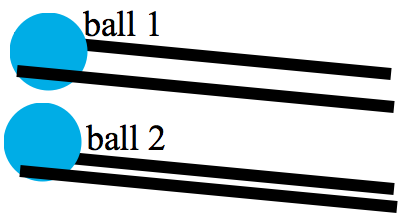
\includegraphics[width=0.25\textwidth]{act214-ramps}
\end{center}

\noindent Your instructor will give you two Pool balls. Let them roll down the channels -- starting them at the same time -- and observe what happens. Do this several times, carefully observing what is different about the way the balls roll. Could the difference be an indication that there is a new energy system that we need to take into account?
\note{\textbf{General Notes}}{
Do not let them bog down in the mechanics of what makes the rotation of the ball on the widely spaced rails faster unless they finish early. The issue may be interesting, but is outside the scope of the Energy-Interaction Model.   Also, don�t worry about the fine details of $KE_{rotation}$.  What�s important is that the indicator is the rotational speed and more of it means more $KE_{rotation}$.  
}

A maybe obvious question is, \textbf{\emph{``Why does one ball go faster and get to the bottom before the other ball?''}} Use the \EnergyInteractionModel{} to make sense of what is going on, and develop a succinct explanation with an appropriate \EnergyDiagram{} for why one of the balls gets to the bottom of the rails before the other ball.

\textbf{Note:} From careful measurements made on this apparatus, friction plays only a very small roll in the difference in speeds of the balls. You can safely assume that all frictional effects cause negligible energy changes compared to the changes in mechanical energies. 
\note{\textbf{Specific Notes}}{
They need to start off making two separate energy system diagrams:     Ball 1 and Ball 2 \\[0.25in]
Make suggestions to the groups at their boards.  One way is to have slower groups, or groups who need more scaffolding, look at the boards of groups who are getting it.
\begin{itemize}
\item	They should conclude that having just the two energy systems isn�t sufficient.  There must be some other energy system involved.
\item Another indicator that can be observed is how fast each ball is rotating, i.e., the rotational speed of each ball.
\item Need to add a rotational kinetic energy system for each ball.
\item There is a difference in the final value of the indicator of rotational KE for each ball.
\item Each diagram now has three energy systems
\item They both have the same decrease in $PE_{grav}$, and they are both closed systems (the earth is automatically a physical object included in the physical system any time the particular model includes $PE_{grav}$).  Ball 1 has a larger change in $KE_{ROT}$, so there is less energy available to go into $KE_{TRANS}$ , meaning less speed.
Congratulate the groups who are able to do this on their own.  Encourage others to go back and work on it at home, so they can do it on their own.
\end{itemize}
}
\WCD